\section{Fusion Evaluation measurement}
I now will list value of different evaluation metrics stated in chapter:6 for different value of sigma for different type of image given in Fig.\ref{fig:6.1}.First i will go with multifocus image and fusion result will shown for pair of image and evaluation metrics will give in table for different method \hfill\break

\begin{figure}[h!]
  \centering
  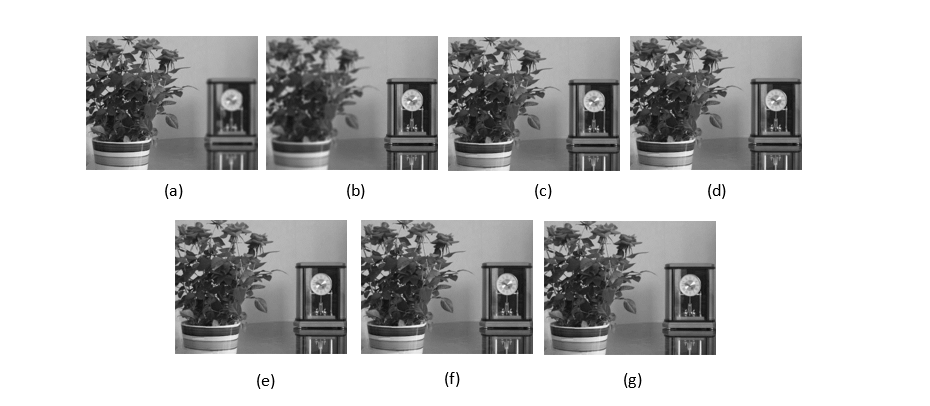
\includegraphics[width=0.9\textwidth]{fus1.png}
  \caption{Example of multifocus image fusion (a)(b) is source image (c)(d)(e)(f)(g) are fusion result for LP-SR, DWR-SR, DTCWT-ST, CVT-SR, NSCT-SR respectivley }\label{fus1}
\end{figure} 
The following table show the evaluation metrics for the above images is given in tabel\ref{tab1}

\begin{table}[!htb] 
 \centering
  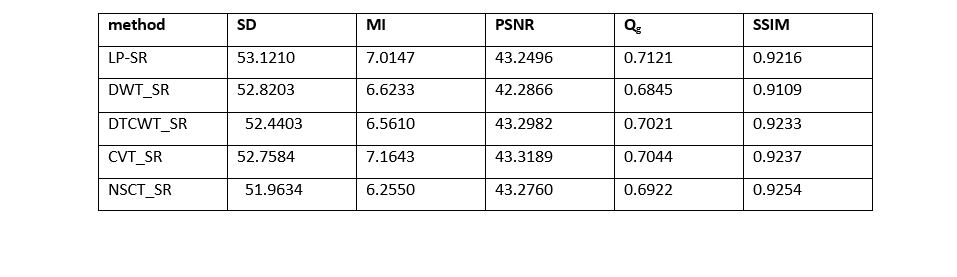
\includegraphics[width=.9\textwidth]{tab1.PNG}
  \caption{Evaluation metrics for different method}
  \label{tab1}
\end{table}

\begin{figure}[h!]
  \centering
  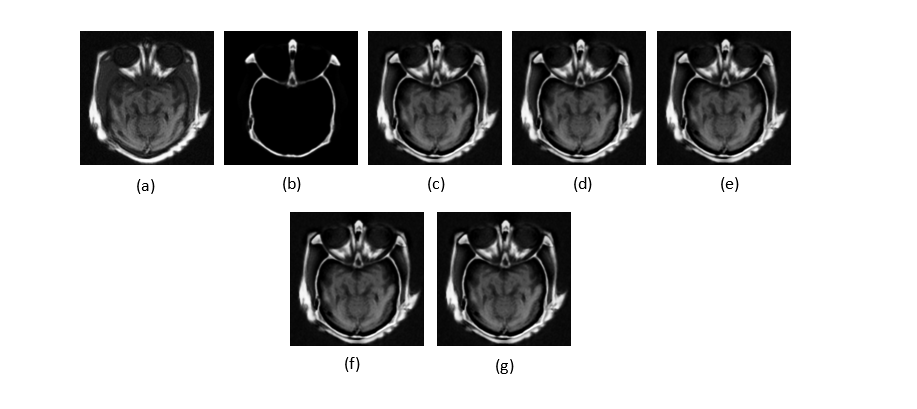
\includegraphics[width=.9\textwidth]{fus2.png}
  \caption{Example of  image fusion (a)MR(b)CT are source images (c)(d)(e)(f)(g) are fusion result for LP-SR, DWR-SR, DTCWT-ST, CVT-SR, NSCT-SR respectivley }\label{fus2}
\end{figure}

The evaluation metrics for different method for medical image is given in table\ref{tab2}

\begin{table}[!htb] 
 \centering
  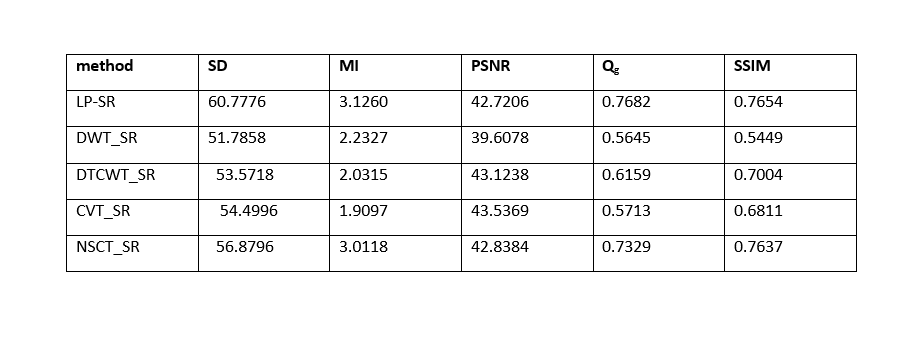
\includegraphics[width=.9\textwidth]{tab2.PNG}
  \caption{Evaluation metrics for different method for medical image}
  \label{tab2}
\end{table}

\begin{figure}[h!]
  \centering
  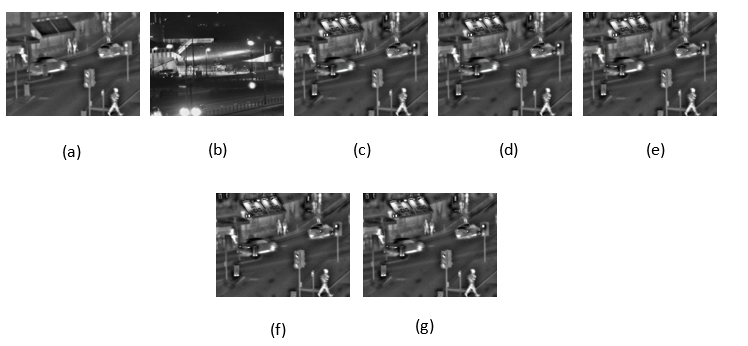
\includegraphics[width=.9\textwidth]{fus3.png}
  \caption{Example of  image fusion (a)infrared image(b)visible image are source images (c)(d)(e)(f)(g) are fusion result for LP-SR, DWR-SR, DTCWT-ST, CVT-SR, NSCT-SR respectivley }\label{fus3}
\end{figure}

The evaluation metrics for different method for visible infrared image is given in table\ref{tab3}

\begin{table}[!htb] 
 \centering
  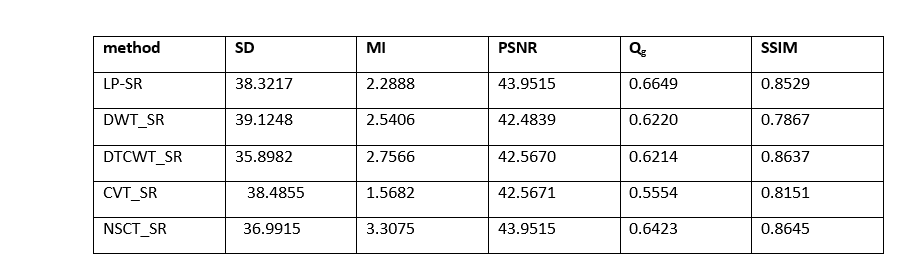
\includegraphics[width=.9\textwidth]{tab3.PNG}
  \caption{Evaluation metrics of different method for infrared image}
  \label{tab3}
\end{table}

Since now we give the experimental result that gives without the noise.When we add noise then how the \textbf{PSNR}  value varies with different values of \textbf{Sigma} is comparatively shown in fig\ref{graph1} for different \textbf{MST} method.I also put the value of psnr in Tabel.\ref{tab4} for multifocus image in Table\ref{tab5} for medical image and in Table\ref{tab6} for infrared image.  

\begin{table}[!htb] 
 \centering
  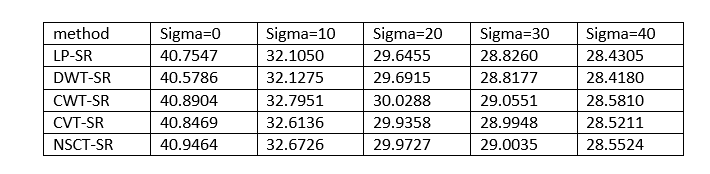
\includegraphics[width=.9\textwidth]{tab4.PNG}
  \caption{PSNR variation for different value of sigma for different method for multifocus image}
  \label{tab4}
\end{table}

\begin{figure}[h!]
  \centering
  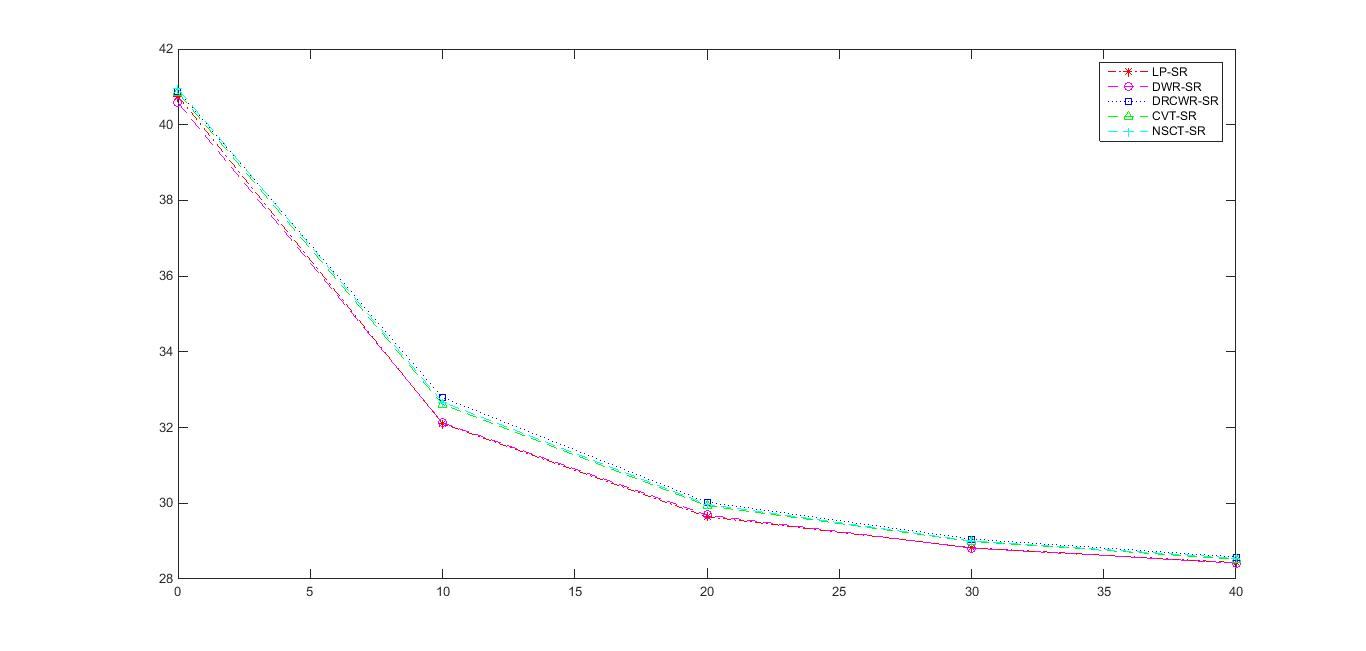
\includegraphics[width=.9\textwidth]{noisevar1.jpg}
  \caption{PSNR variation for different value of sigma for multifocus image of first image pair shown in figure \ref{fig:6.1}}\label{graph1}
\end{figure}

\begin{table}[!htb] 
 \centering
  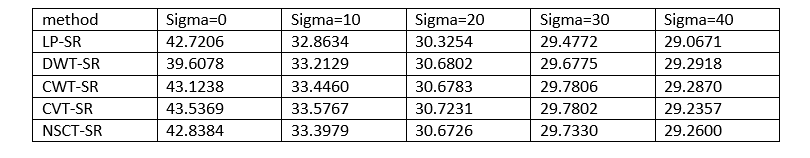
\includegraphics[width=.9\textwidth]{tab5.PNG}
  \caption{PSNR variation for different value of sigma for different method for medical image}
  \label{tab5}
\end{table}

\begin{figure}[h!]
  \centering
  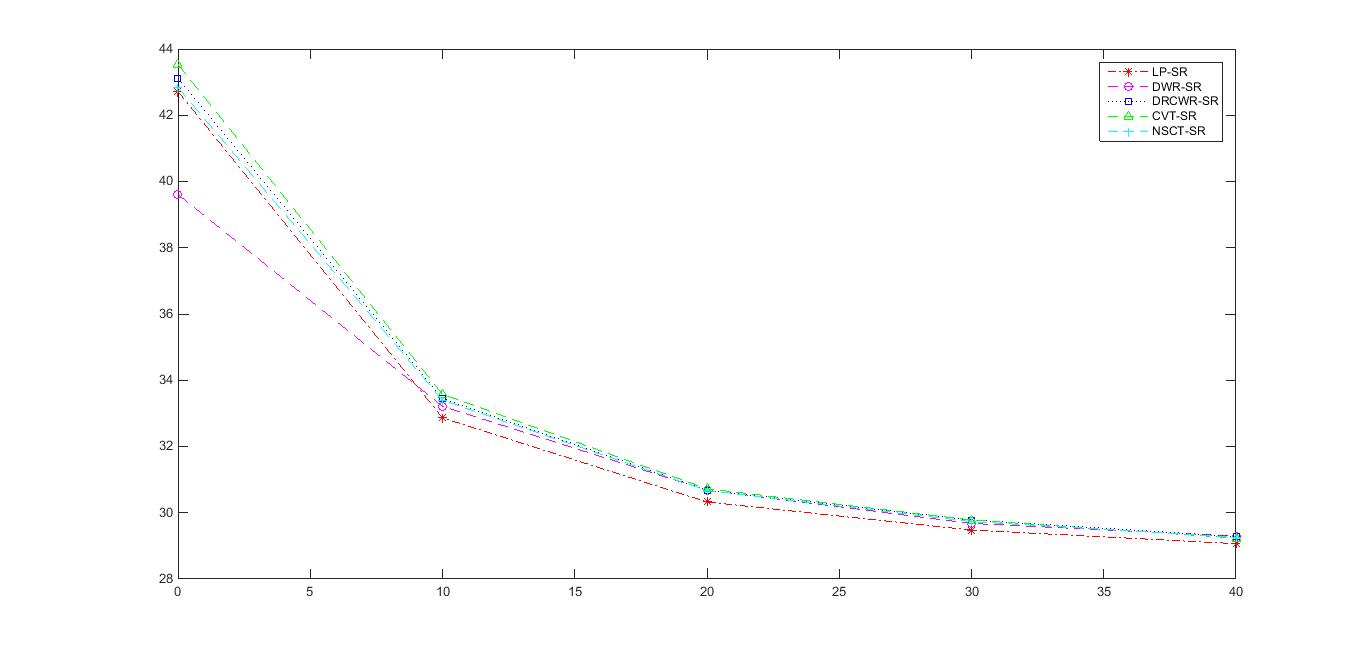
\includegraphics[width=.9\textwidth]{noisevar2.jpg}
  \caption{PSNR variation for different value of sigma for medical image of first medical image image pair shown in figure \ref{fig:6.1}}
  \label{graph2}
\end{figure}

\section{Discussion}
 for each type of image fusion, I take the related contents in Tables \ref{tab1}-\ref{tab5} into consideration together and seek out some common regularities among the six MST s used in the proposed framework. \hfill \break
 
 From the data obtained from table\ref{tab1}-\ref{tab5} and graph\ref{graph1}-\ref{graph2} we see that NSCT-SR based image fusion gives better result than other method.We perform this task on about 50 pair of image and this method gives the better result than any others method. 


